%%%%%%%%%%%%%%%%%%%%%%%%%%%%%%%%%%%%%%%%%%%%%%%%%%%%%%%%%%%%%%%%%%%%%%%%%%%%%%%%%%%%%%
%% Author:      Nils Weber and Maximilian Stiefel
%% Date:        23.12.2017
%% University:  Uppsala Universitet
%% Department:  Institutionen för informationsteknologi 
%% Course:      Embedded Control System Project
%% Project:     PRECISELY CONTROLLED DIY ETCHING MACHINE 
%%				FOR USAGE AT HOME AND IN SMALL LABS
%%%%%%%%%%%%%%%%%%%%%%%%%%%%%%%%%%%%%%%%%%%%%%%%%%%%%%%%%%%%%%%%%%%%%%%%%%%%%%%%%%%%%%

\chapter{Introduction} 
\label{chap:introduction} 
At some point in the career an embedded systems engineer needs a quick hardware prototype. One had an idea and wants to try it out. With modern \gls{ECAD} software the \gls{PCB} design is ready within a week or even less. Leading electronic component distributors also guarantee delivery within an acceptable timespan of a few days. However, the preferred \gls{PCB} manufacturer most likely needs a week for the manufacturing and another week for shipping. For this reason, if time is a limited resource, \gls{DIY} etching in the lab can be an option to consider. 

\begin{figure}[H]                                                         
\centering          
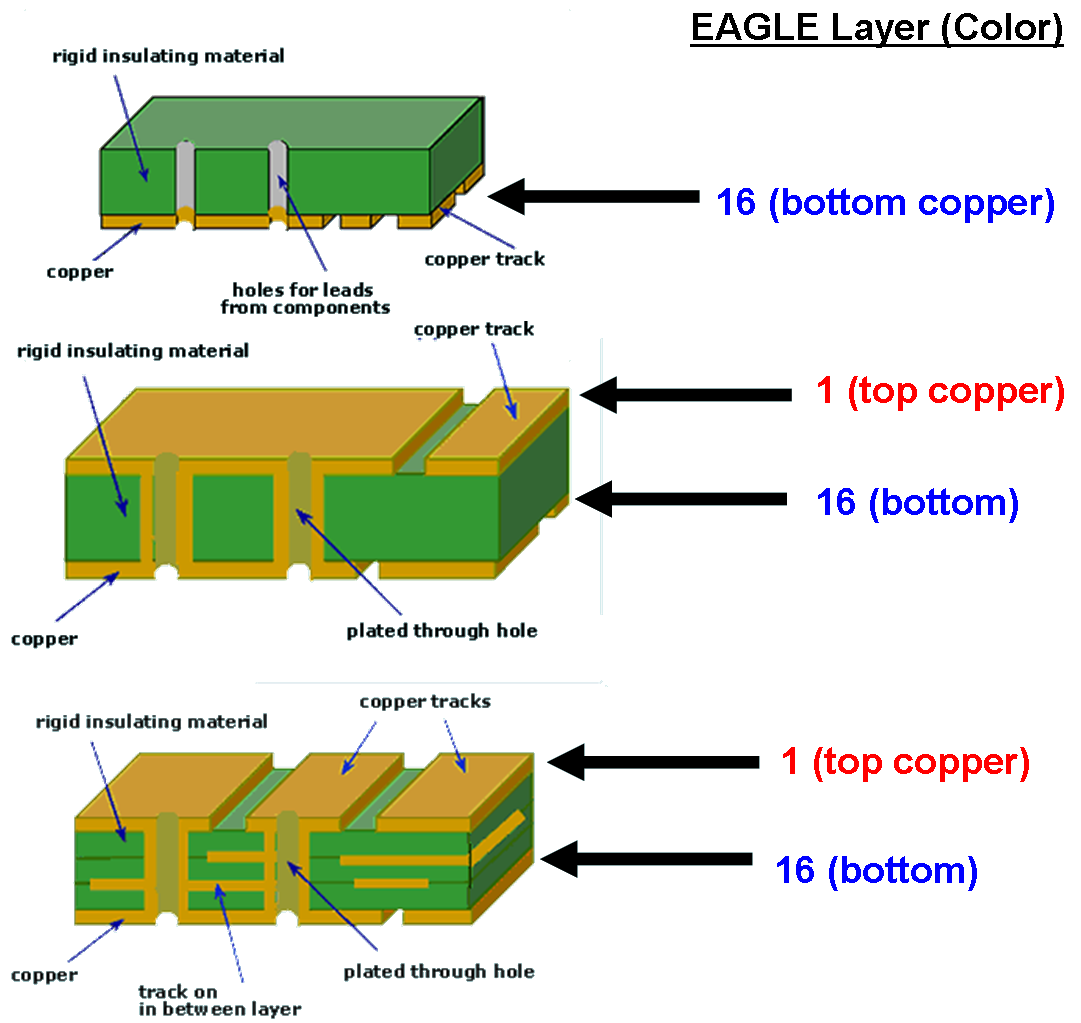
\includegraphics[width=0.7\textwidth]{./fig/PCBLayers}   
\caption[Layered structure of \glspl{PCB}.]{Layered structure of \glspl{PCB}. Top: 1 layer. Middle: 2 layers. Bottom: 4 layers. Source: \cite{online:pcblayers}}   
\label{fig:pcblayers}                                                       
\end{figure}  

A \gls{PCB} basically consists out of copper layers, substrate layers and vias to interconnect different layers (cf. fig. \ref{fig:pcblayers}). There are three different kind of vias in modern electronics:
\begin{enumerate}
\item Through-hole vias as one can see in fig. \ref{fig:pcblayers}
\item Blind vias, which only connect an outer layer to one (or multiple) inner layers
\item Buried vias, which connect two copper layers inside
\end{enumerate}
Blind and buried vias can be implemented as micro vias, which means nothing, but that they are very small, because a laser is used to melt two layers together in a tiny (\ensuremath{<} \SI{0.1}{\milli\metre}) circular area. Conventional \gls{DIY} etching techniques only support the first option. The other two options are usually nowadays still more expensive than normal through-hole vias, which have been around for quite some time already.  Without reservations, using a \gls{DIY} approach, \glspl{PCB} with a complexity of two layers can be crafted nowadays. The basic idea of \gls{DIY} \gls{PCB} crafting is to remove the copper from a blank in certain areas to obtain the desired layout. Distributors nowadays offer blanks with one or two layers and substrate (with a thickness of usually \SI{1.6}{\milli\metre}). Most common is the format \SI{100}{\milli\metre} x \SI{160}{\milli\metre} (\myemph{Eurocard}). Taking away the copper can be achieved mechanically and chemically, whereas this work is about the latter.  
\newpar
\gls{DIY} etching is usually done in either of two ways: 
\begin{enumerate}
\item The toner transfer method: The layout is printed on glossy or transparent paper and the toner is transfered with heat to the blank copper board (cf. \cite{online:instructtoner}). There are several severe disadvantages with this method e.g. that it is hard to align the masks for a \gls{PCB} with two layers.  
\item The photoresist method: Photoresist is used to cover the copper completely and then a \gls{UV} lamp in combination with a mask printed on transparency is leveraged to destroy the photoresist, where it is not covered by the black color on the transparency (cf. \cite{online:instructphoto}). The cracked photoresist, which is damaged by \gls{UV} light can then be washed away with sodium hydroxid (NaOH). 
\end{enumerate}
In both cases an etching bath is necessary to etch away the unprotected copper. Popular chemicals to achieve the copper removal are iron(III) chloride ($\text{FeCl}_3$) and sodium persulfate ($\text{Na}_2\text{S}_2\text{O}_8$).
\newpar
Sodium persulfate gives better results i.e. better or finer contours. Moreover, the sodium persulfate etching liquid is transparent blue unlike the liquid with iron(III) chloride, which is brown and non-transparent. Solving sodium persulfate in water results in
\begin{center}
	\ch{Na2S2O8_{(s)} -> 2 Na^{+}_{(aq)} + S2O8^{2-}_{(aq)}}.
\end{center}
In the etching process elemental copper is oxidated to copper ions, which are then a part of the etching liquid. 
\begin{center}
	\ch{S2O8^{2-}_{(aq)} + Cu_{(s)} -> 2 SO4^{2-}_{(aq)} + Cu^{2+}_{(aq)}}
\end{center}
Special care needs to be taken of the etching liquid afterwards. Copper ions are toxic for all kind of organisms. The last step of \gls{PCB} crafting is the drilling. It can be challenging especially if one uses small via sizes (down to \SI{0.2}{\milli\metre} is not uncommon). One also has to find solution or rather keep in mind, that a via is supposed to interconnect different \gls{PCB} layers, which is hard to achieve creating \gls{PCB} in a \gls{DIY} manner as one somehow has to plate the inside of the cylindric via drill hole with copper in order to create a genuine via.   
% Write what we opt to achieve with this project.
\newpar 
The goal of this project is to develop cheap and easy-to-use etching equipment for the photoresist method. It shall be very easy for engineers to replicate the equipment and also to even tailor it. All the design files shall be open and available on the net. 
\newpar
In principle, what is necessary to start crafting prototypes, is an etching tank and a \gls{UV} light source. Both are subject to what this project opts to achieve as a result.   
\newpar 
The whole project is pushed regularly on \myemph{Github}: \href{https://github.com/m3x1m0m/EmbeddedEtcher}{https://github.com/m3x1m0m/EmbeddedEtcher}